\documentclass[tikz,border=0pt]{standalone}
\usepackage{iftex}
\ifLuaTeX
\usepackage{fontspec}
\setsansfont{DejaVu Sans}
\else
\usepackage[T1]{fontenc}
\usepackage[utf8]{inputenc}
\usepackage{lmodern}
\fi
\usepackage{amsmath}
\usetikzlibrary{arrows.meta}
\renewcommand{\familydefault}{\sfdefault}
\definecolor{adbg}{HTML}{101827}
\definecolor{adfg}{HTML}{F1F5F9}
\definecolor{admuted}{HTML}{B5C4D9}
\definecolor{adline}{HTML}{A9BDD8}
\definecolor{adgroup}{HTML}{172236}
\definecolor{adborder}{HTML}{435470}
\definecolor{adinput}{HTML}{93C5FD}
\definecolor{adinputfill}{HTML}{202E44}
\definecolor{adcompute}{HTML}{5EEAD4}
\definecolor{adcomputefill}{HTML}{202E44}
\definecolor{admodel}{HTML}{C4B5FD}
\definecolor{admodelfill}{HTML}{202E44}
\definecolor{admemory}{HTML}{7DD3FC}
\definecolor{admemoryfill}{HTML}{202E44}
\definecolor{adtool}{HTML}{FCD34D}
\definecolor{adtoolfill}{HTML}{202E44}
\definecolor{adcontrol}{HTML}{CBD5E1}
\definecolor{adcontrolfill}{HTML}{202E44}
\definecolor{adoutput}{HTML}{6EE7B7}
\definecolor{adoutputfill}{HTML}{202E44}
\definecolor{adneutral}{HTML}{CBD5E1}
\definecolor{adneutralfill}{HTML}{202E44}
\begin{document}
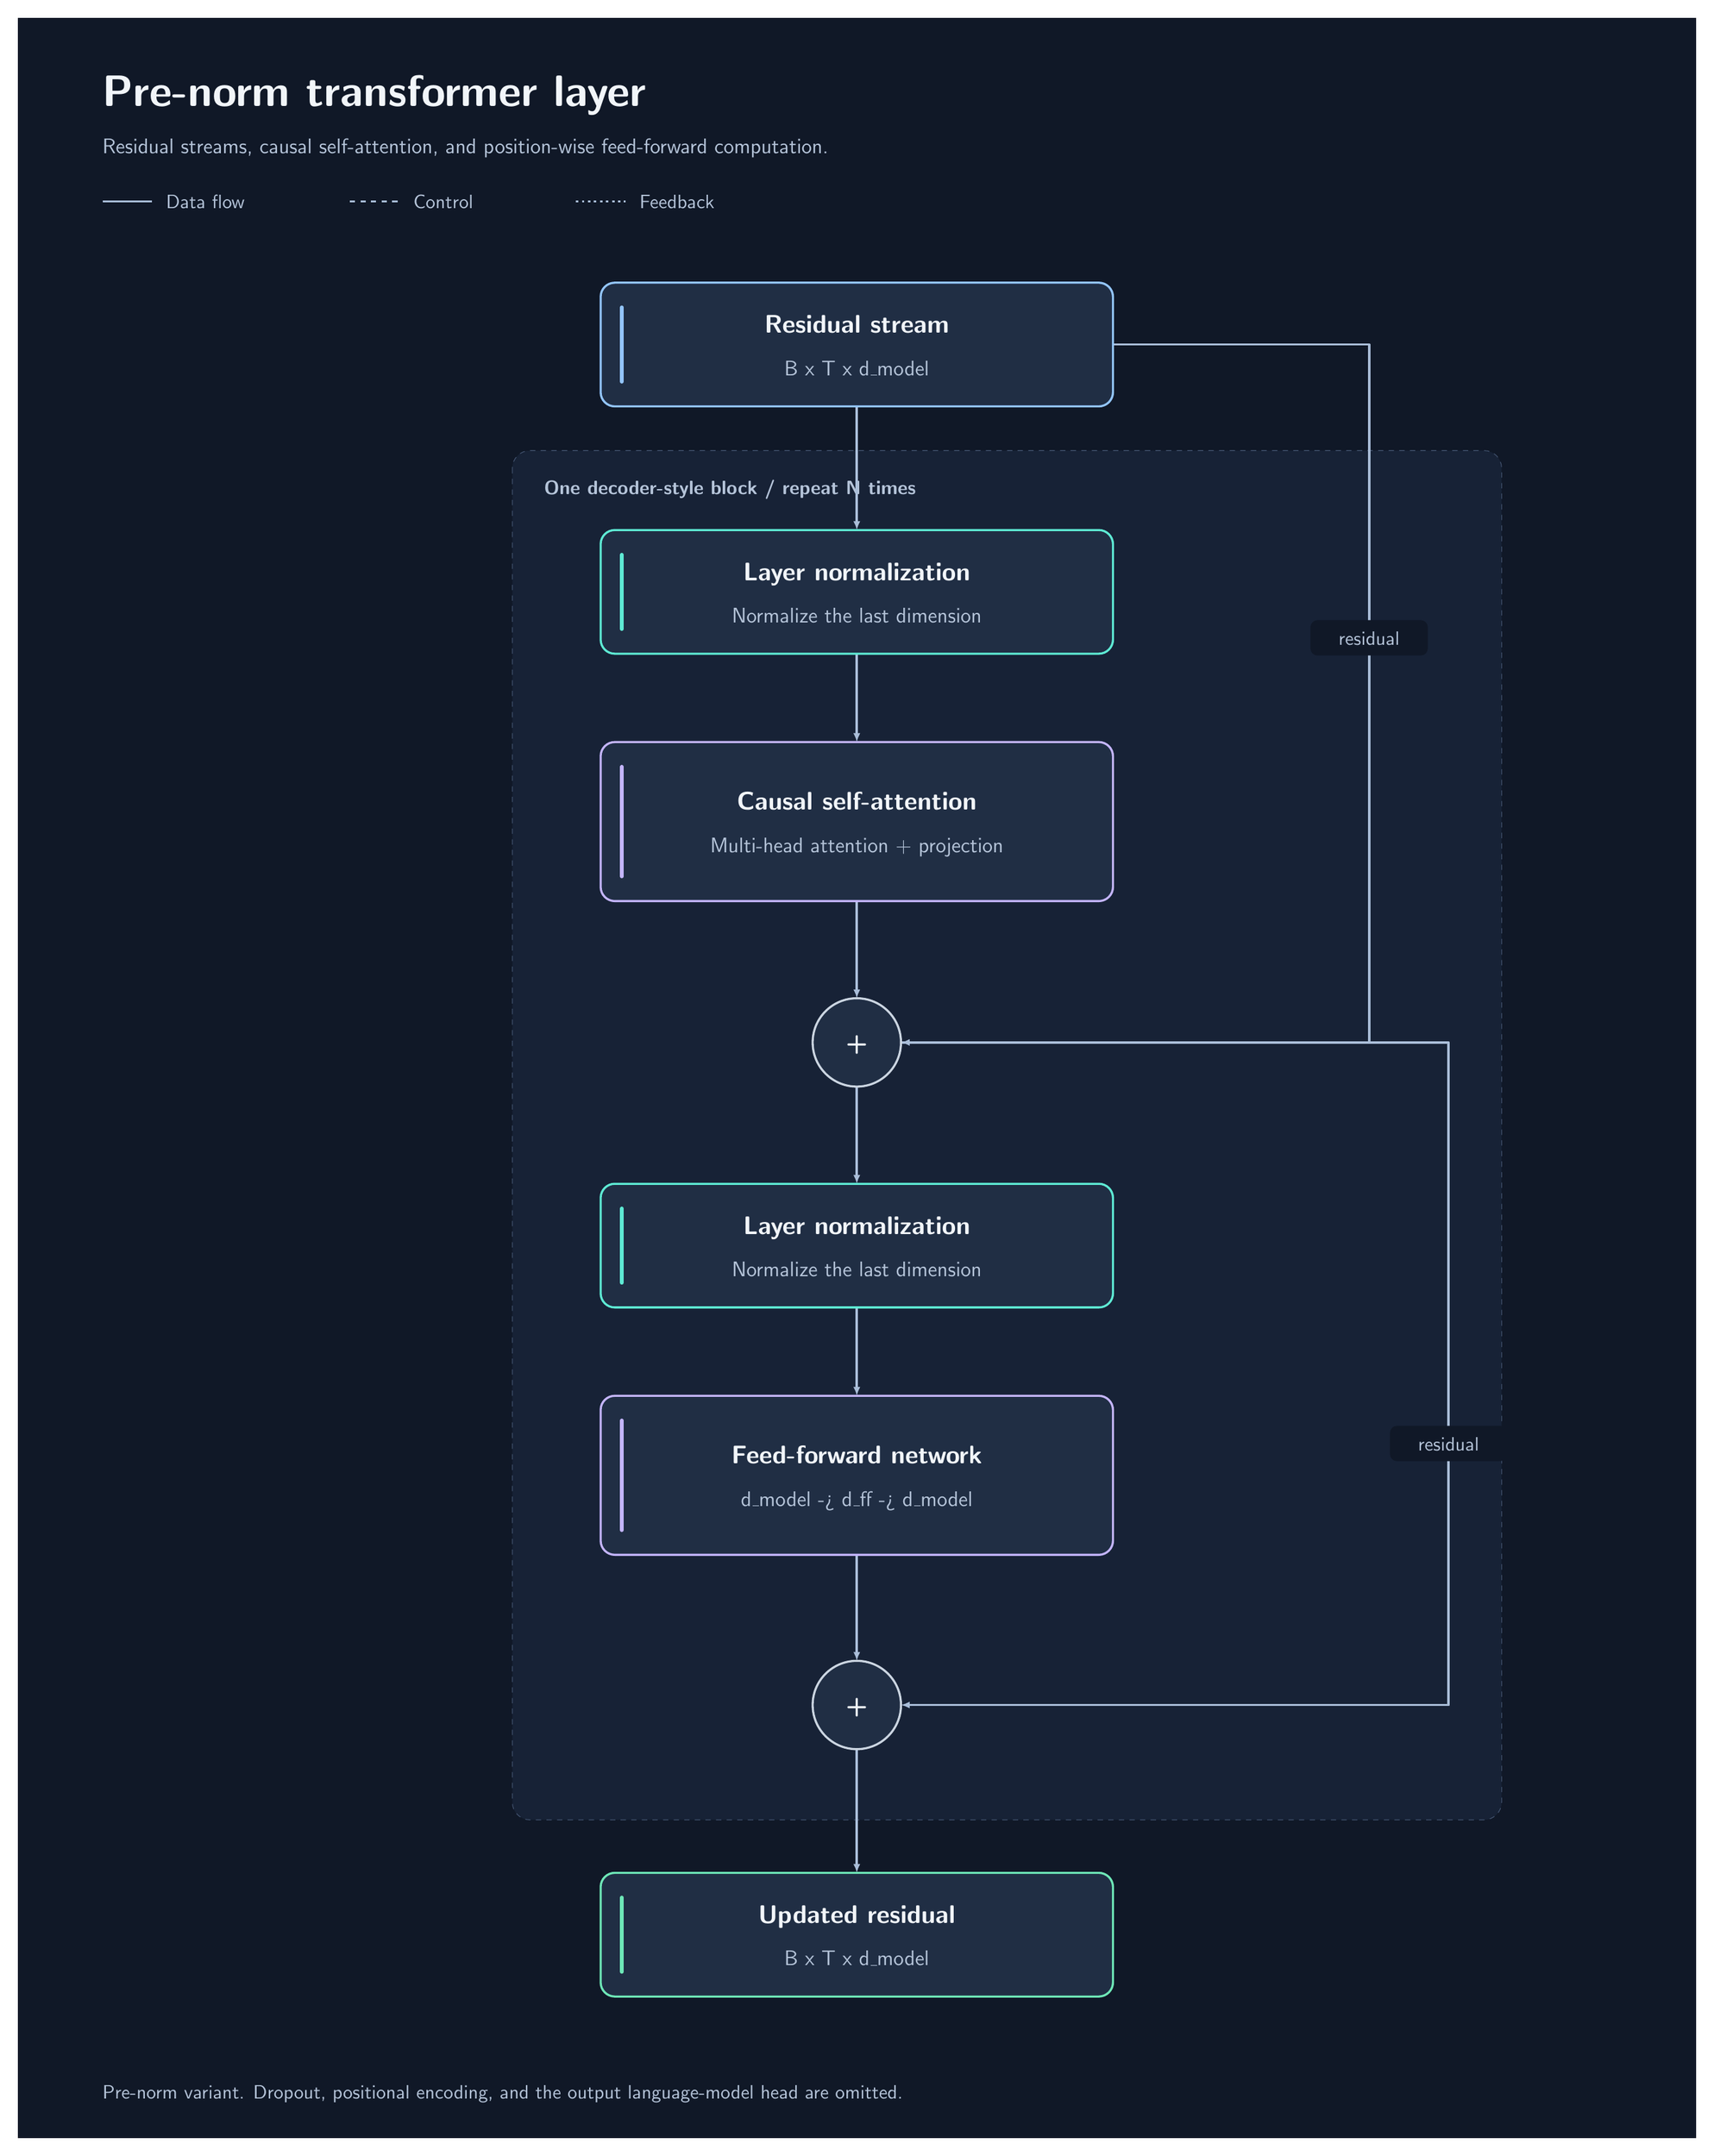
\begin{tikzpicture}[x=1pt,y=-1pt,inner sep=0pt,outer sep=0pt]
\path[use as bounding box] (0,0) rectangle (950,1200);
\fill[adbg] (0,0) rectangle (950,1200);
\node[anchor=base west,text=adfg,font={\sffamily\fontsize{29}{34.8}\selectfont\bfseries}] at (48,50) {Pre-norm transformer layer};
\node[anchor=base west,text=admuted,font={\sffamily\fontsize{13}{15.6}\selectfont}] at (48,77) {Residual streams, causal self-attention, and position-wise feed-forward computation.};
\draw[adline,line width=1.4pt] (48,104) -- (76,104);
\node[anchor=base west,text=admuted,font={\sffamily\fontsize{10.5}{12.6}\selectfont}] at (84,108) {Data flow};
\draw[adline,line width=1.4pt,dashed] (188,104) -- (216,104);
\node[anchor=base west,text=admuted,font={\sffamily\fontsize{10.5}{12.6}\selectfont}] at (224,108) {Control};
\draw[adline,line width=1.4pt,dotted] (316,104) -- (344,104);
\node[anchor=base west,text=admuted,font={\sffamily\fontsize{10.5}{12.6}\selectfont}] at (352,108) {Feedback};
\draw[fill=adgroup,draw=adborder,dashed,rounded corners=10pt] (280,245) rectangle (840,1020);
\node[anchor=base west,text=admuted,font={\sffamily\fontsize{11}{13.2}\selectfont\bfseries}] at (298,270) {One decoder-style block / repeat N times};
\draw[adline,line width=1.3pt,-{Latex[length=5pt,width=4pt]},line join=round] (475,220) -- (475,255) -- (475,290);
\draw[adline,line width=1.3pt,-{Latex[length=5pt,width=4pt]},line join=round] (475,360) -- (475,385) -- (475,410);
\draw[adline,line width=1.3pt,-{Latex[length=5pt,width=4pt]},line join=round] (475,500) -- (475,527.5) -- (475,555);
\draw[adline,line width=1.3pt,-{Latex[length=5pt,width=4pt]},line join=round] (475,605) -- (475,632.5) -- (475,660);
\draw[adline,line width=1.3pt,-{Latex[length=5pt,width=4pt]},line join=round] (475,730) -- (475,755) -- (475,780);
\draw[adline,line width=1.3pt,-{Latex[length=5pt,width=4pt]},line join=round] (475,870) -- (475,900) -- (475,930);
\draw[adline,line width=1.3pt,-{Latex[length=5pt,width=4pt]},line join=round] (475,980) -- (475,1015) -- (475,1050);
\draw[adline,line width=1.3pt,-{Latex[length=5pt,width=4pt]},line join=round] (620,185) -- (765,185) -- (765,580) -- (500,580);
\draw[adline,line width=1.3pt,-{Latex[length=5pt,width=4pt]},line join=round] (500,580) -- (810,580) -- (810,955) -- (500,955);
\draw[draw=adinput,fill=adinputfill,line width=1.2pt,rounded corners=8pt] (330,150) rectangle (620,220);
\draw[adinput,line width=2.2pt,line cap=round] (342,164) -- (342,206);
\node[anchor=base,text=adfg,font={\sffamily\fontsize{15}{18.0}\selectfont\bfseries}] at (475,178.5) {Residual stream};
\node[anchor=base,text=admuted,font={\sffamily\fontsize{11.5}{13.799999999999999}\selectfont}] at (475,202.5) {B x T x d\_model};
\draw[draw=adcompute,fill=adcomputefill,line width=1.2pt,rounded corners=8pt] (330,290) rectangle (620,360);
\draw[adcompute,line width=2.2pt,line cap=round] (342,304) -- (342,346);
\node[anchor=base,text=adfg,font={\sffamily\fontsize{15}{18.0}\selectfont\bfseries}] at (475,318.5) {Layer normalization};
\node[anchor=base,text=admuted,font={\sffamily\fontsize{11.5}{13.799999999999999}\selectfont}] at (475,342.5) {Normalize the last dimension};
\draw[draw=admodel,fill=admodelfill,line width=1.2pt,rounded corners=8pt] (330,410) rectangle (620,500);
\draw[admodel,line width=2.2pt,line cap=round] (342,424) -- (342,486);
\node[anchor=base,text=adfg,font={\sffamily\fontsize{15}{18.0}\selectfont\bfseries}] at (475,448.5) {Causal self-attention};
\node[anchor=base,text=admuted,font={\sffamily\fontsize{11.5}{13.799999999999999}\selectfont}] at (475,472.5) {Multi-head attention + projection};
\draw[draw=adcontrol,fill=adcontrolfill,line width=1.2pt] (475,580) ellipse [x radius=25pt,y radius=25pt];
\node[anchor=base,text=adfg,font={\sffamily\fontsize{15}{18.0}\selectfont\bfseries}] at (475,585) {+};
\draw[draw=adcompute,fill=adcomputefill,line width=1.2pt,rounded corners=8pt] (330,660) rectangle (620,730);
\draw[adcompute,line width=2.2pt,line cap=round] (342,674) -- (342,716);
\node[anchor=base,text=adfg,font={\sffamily\fontsize{15}{18.0}\selectfont\bfseries}] at (475,688.5) {Layer normalization};
\node[anchor=base,text=admuted,font={\sffamily\fontsize{11.5}{13.799999999999999}\selectfont}] at (475,712.5) {Normalize the last dimension};
\draw[draw=admodel,fill=admodelfill,line width=1.2pt,rounded corners=8pt] (330,780) rectangle (620,870);
\draw[admodel,line width=2.2pt,line cap=round] (342,794) -- (342,856);
\node[anchor=base,text=adfg,font={\sffamily\fontsize{15}{18.0}\selectfont\bfseries}] at (475,818.5) {Feed-forward network};
\node[anchor=base,text=admuted,font={\sffamily\fontsize{11.5}{13.799999999999999}\selectfont}] at (475,842.5) {d\_model -> d\_ff -> d\_model};
\draw[draw=adcontrol,fill=adcontrolfill,line width=1.2pt] (475,955) ellipse [x radius=25pt,y radius=25pt];
\node[anchor=base,text=adfg,font={\sffamily\fontsize{15}{18.0}\selectfont\bfseries}] at (475,960) {+};
\draw[draw=adoutput,fill=adoutputfill,line width=1.2pt,rounded corners=8pt] (330,1050) rectangle (620,1120);
\draw[adoutput,line width=2.2pt,line cap=round] (342,1064) -- (342,1106);
\node[anchor=base,text=adfg,font={\sffamily\fontsize{15}{18.0}\selectfont\bfseries}] at (475,1078.5) {Updated residual};
\node[anchor=base,text=admuted,font={\sffamily\fontsize{11.5}{13.799999999999999}\selectfont}] at (475,1102.5) {B x T x d\_model};
\fill[adbg,rounded corners=4pt] (731.8,341) rectangle (798.2,361);
\node[anchor=base,text=admuted,font={\sffamily\fontsize{11}{13.2}\selectfont}] at (765,355) {residual};
\fill[adbg,rounded corners=4pt] (776.8,797) rectangle (843.2,817);
\node[anchor=base,text=admuted,font={\sffamily\fontsize{11}{13.2}\selectfont}] at (810,811) {residual};
\node[anchor=base west,text=admuted,font={\sffamily\fontsize{11}{13.2}\selectfont}] at (48,1178) {Pre-norm variant. Dropout, positional encoding, and the output language-model head are omitted.};
\end{tikzpicture}
\end{document}
